\documentclass{beamer}

% to include graphics
\usepackage{graphicx}

% to include hyperlinks
\usepackage{hyperref}

% divide slides into columns
\usepackage{multicol}


\usetheme{Copenhagen}
\usecolortheme{beaver}

\usepackage{graphicx}
\usepackage{subcaption}

\title{Cluster Progress}
\date{\today}

\begin{document}

%----------BEGIN TITLE----------

\begin{frame}
  \maketitle
\end{frame}

%-----------END TITLE-----------

%----------BEGIN NAS-1----------

\begin{frame}
  \frametitle{NAS-1 Progress}

  \begin{itemize}    
  \item NAS-1 no longer boots into emergency mode. 
  \item The hard drive in slot 0:21 is currently rebuilding, all others are online.   
  \end{itemize}
  % this happened after Michael and I took nas1 out (twice) to check for a model number on the raid card
  %even though you can see that on boot and by running a command...
  %not sure what was wrong and what fixed it but it's fixed now
  \begin{figure}[H]
    \begin{center}
      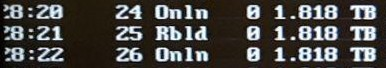
\includegraphics[width=0.5\textwidth]{nas1_drives_status.jpg}
    \end{center}
  \end{figure}

  \begin{figure}[H]
    \begin{center}
      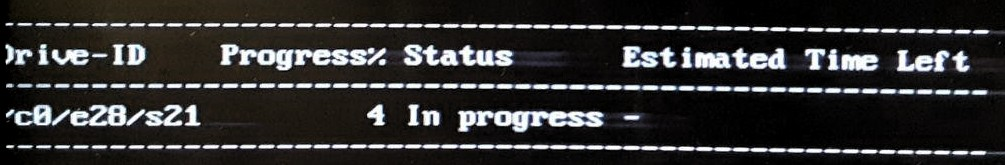
\includegraphics[width=0.5\textwidth]{nas1_drive21_rebuild.jpg}
    \end{center}
  \end{figure}
  

\end{frame}
%-----------END NAS-1-----------

%---------BEGIN NAS-0-----------
\begin{frame}
  \frametitle{NAS-0 ZFS}

  \begin{itemize}
  \item Somehow, zfs was uninstalled from NAS-0, as well as twcli.
  \item twcli has been reinstalled successfully, but zfs is having issues reinstalling.
  \item Once they are reinstalled, hopefully the zpool can be discovered and reimported.   
  \end{itemize}
  
\end{frame}
%-----------END NAS-0-----------

%zfs - filesystem and logical volume manager - ``software raid'' -nas0 drives in the zpool\\
%tw_cli - raid monitoring software - controller, logical unit, drive management\\

%---------BEGIN APC-UPS---------
\begin{frame}
  \frametitle{APC Batteries}

  \begin{itemize}
  \item The voltages on the APC batteries have dropped from 12.5V to ~9V (and some almost to 0)
  \item New batteries have been ordered and should be delivered soon.    
  \end{itemize}

\end{frame}
%-----------END APC-UPS---------

%t3 cluster meetings: need to get access to lxplus to sign up, and CERN lightweight acct doesnt have accest to lxplus.
% solution: contact  former secretariat and renew my affiliation

%OSG: provided me a link to the guide on how to renew host certs, but no word back yet on my account status. 

\end{document}
